\documentclass[aspectratio=169]{beamer}
\usepackage{will_handley_beamer}

% Commands
% --------
% - \arxiv{arxiv number}
% - \cols{width}{lh column}{rh column}
% -  \begin{fig(left|right)}[fractional width (e.g 0.6) ]{name of image}
%        content of other column
%    \end{fig(left|right)}

% Talk details
% ------------
\title{Theory, observation \& cosmological inference}
\subtitle{Introduction to KICC: 5 minutes on Will Handley's research}
\date{7\textsuperscript{th} December 2022}

\begin{document}

\begin{frame}
    \titlepage
\end{frame}

\begin{frame}
    \frametitle{Research overview}
    \begin{columns}
        \column{0.3\textwidth}
        \begin{block}{Theory}
            \begin{itemize}
                \item Early universe cosmology
                \item Modified gravity
            \end{itemize}
        \end{block}
        \column{0.3\textwidth}
        \begin{block}{Inference}
            \begin{itemize}
                \item Nested sampling
                \item Likelihood free inference
            \end{itemize}
        \end{block}
        \column{0.3\textwidth}
        \begin{block}{Observation}
            \begin{itemize}
                \item REACH
                \item GAMBIT
            \end{itemize}
        \end{block}
    \end{columns}
    
    \begin{columns}[t]
        \column{0.28\textwidth}
        \begin{block}{\texttt{PolyChord}}
            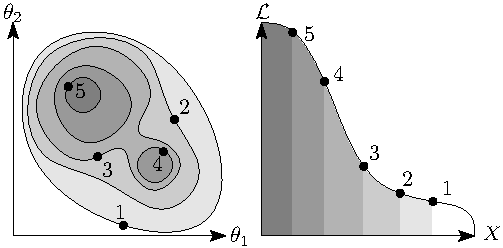
\includegraphics[width=\textwidth]{figures/polychord1.pdf}
            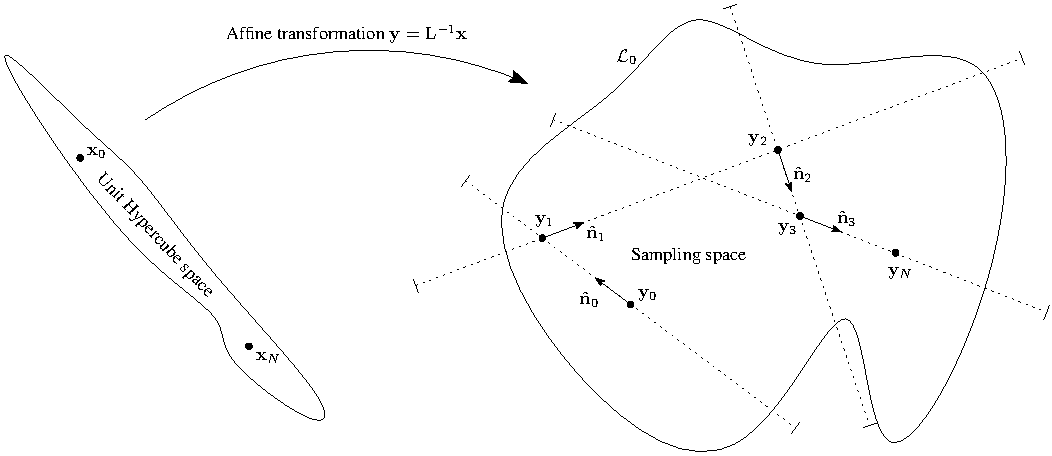
\includegraphics[width=\textwidth]{figures/polychord2.pdf}
        \end{block}
        
        \column{0.35\textwidth}
        \begin{block}{\texttt{fgivenx}}
            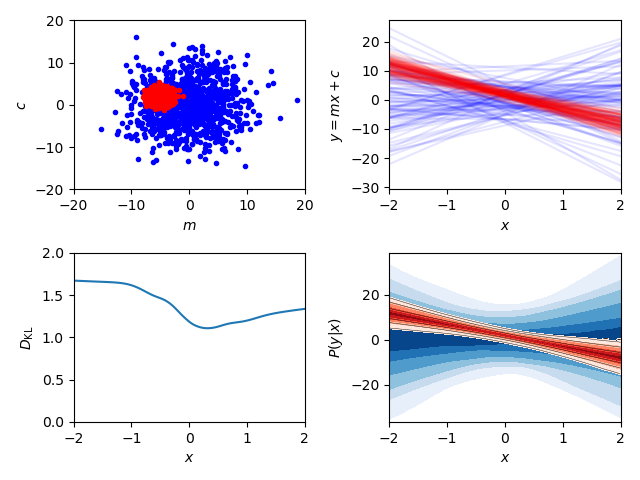
\includegraphics[width=\textwidth]{figures/fgivenx.png}
        \end{block}

        \column{0.22\textwidth}
        \begin{block}{\texttt{anesthetic}}
            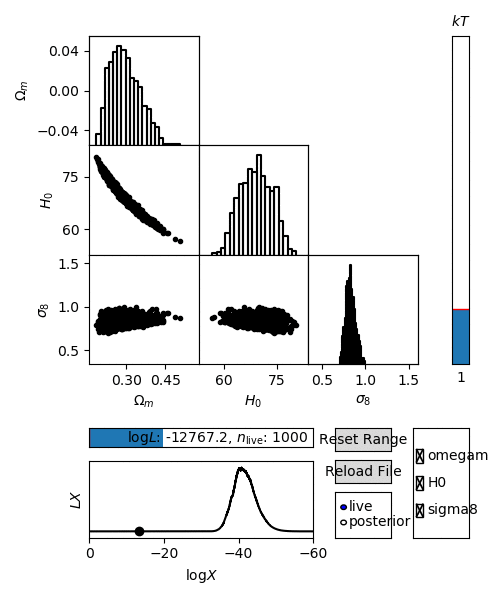
\includegraphics[width=\textwidth]{figures/anim_1-10.png}
        \end{block}
    \end{columns}



    \hfill Coming soon: \texttt{unimpeded}, \texttt{supernest}
\end{frame}

\begin{frame}
    \frametitle{Theory of the primordial and late-time universe}
    \begin{columns}
        \column{0.5\textwidth}
        \small
        \begin{tabular}{lp{5cm}}
            \raisebox{-.8\totalheight}{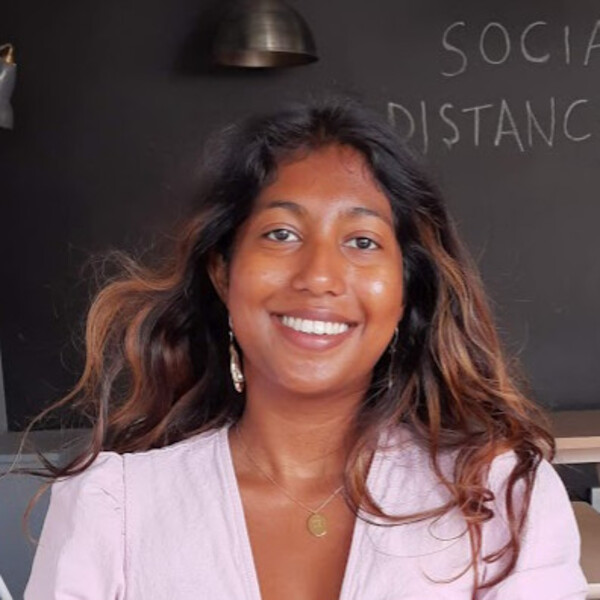
\includegraphics[width=50px]{images/metha_prathaban.jpg}}&
            \textbf{Metha Prathaban} (PhD1) \newline
            Palindromic \& two-sheeted universes -- boundary conditions \& Boltzmann solvers.
            \\

            \raisebox{-.7\totalheight}{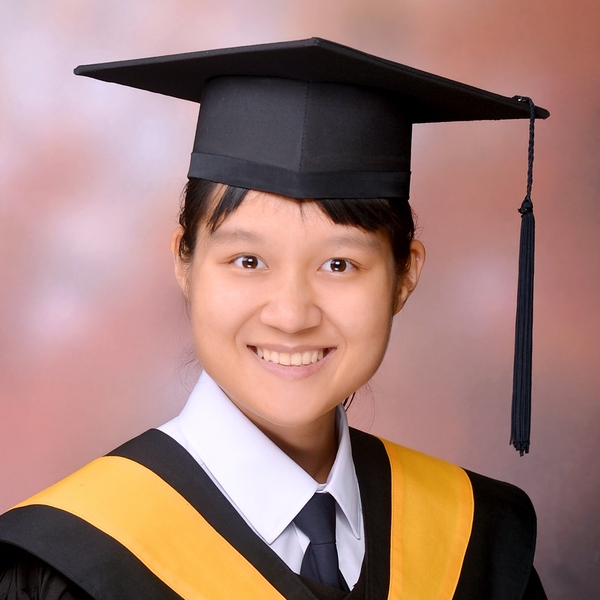
\includegraphics[width=50px]{images/wei-ning_deng.jpg}}&
            \textbf{Wei-Ning Deng} (PhD1) \newline
            Primordial curvature \& comoving curvature perturbations $\mathcal{R}$.
            \\
            \raisebox{-.8\totalheight}{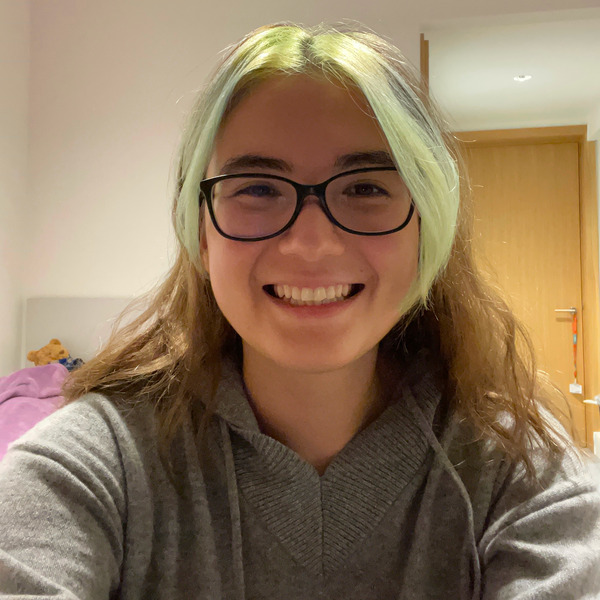
\includegraphics[width=50px]{images/sinah_legner.jpg}}&
            \textbf{Sinah Legner} (PhD1) 
            \raisebox{-.4\totalheight}{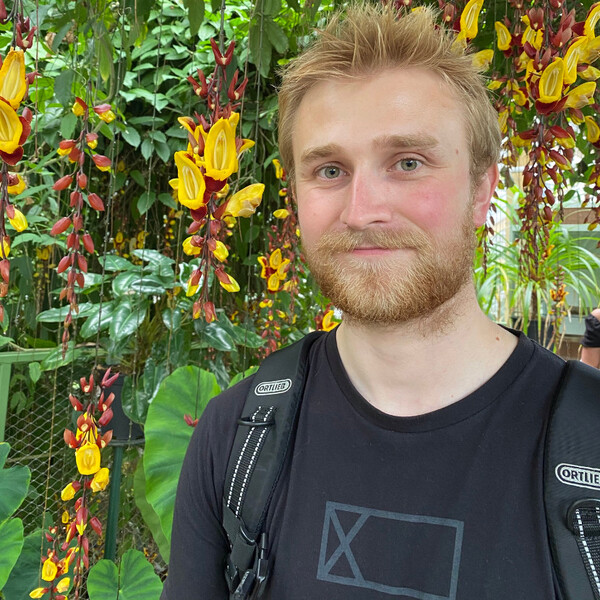
\includegraphics[height=20px]{images/will_barker.jpg}}
            \newline 
            Predictions \& perturbations from gravitational gauge-theories.
            \\

            \raisebox{-.8\totalheight}{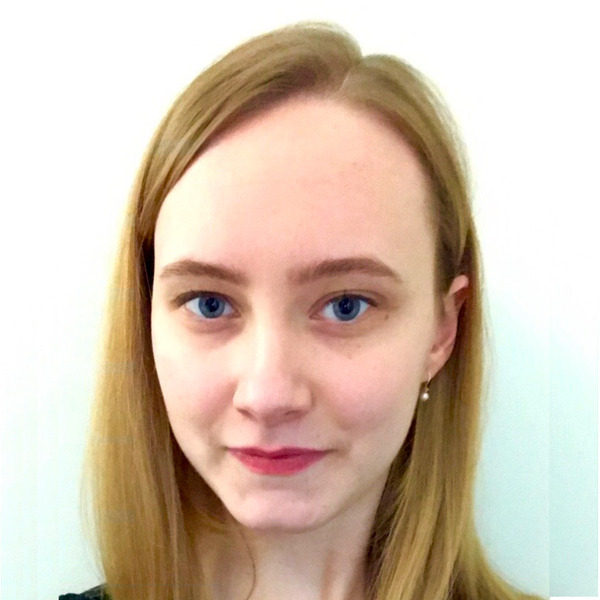
\includegraphics[width=50px]{images/danielle_dineen.jpg}}&
            \textbf{Danielle Dineen} (MPhil) \newline
            Israel junction conditions and potential-independent predictions from inflation.
            \\
        \end{tabular}

        \column{0.5\textwidth}
        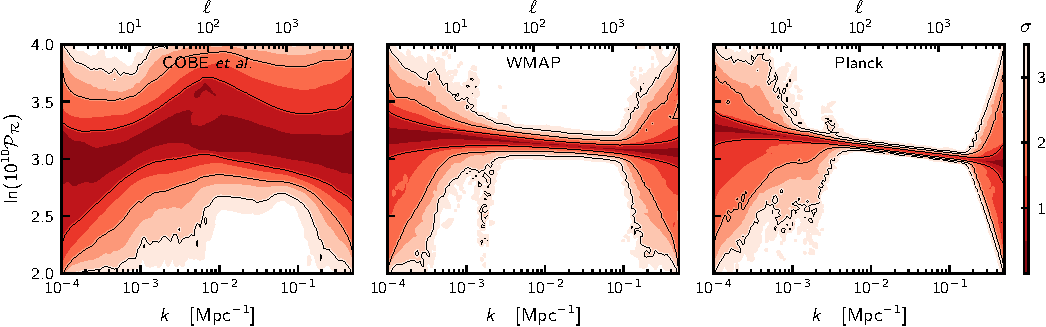
\includegraphics[width=\textwidth]{figures/pps}
        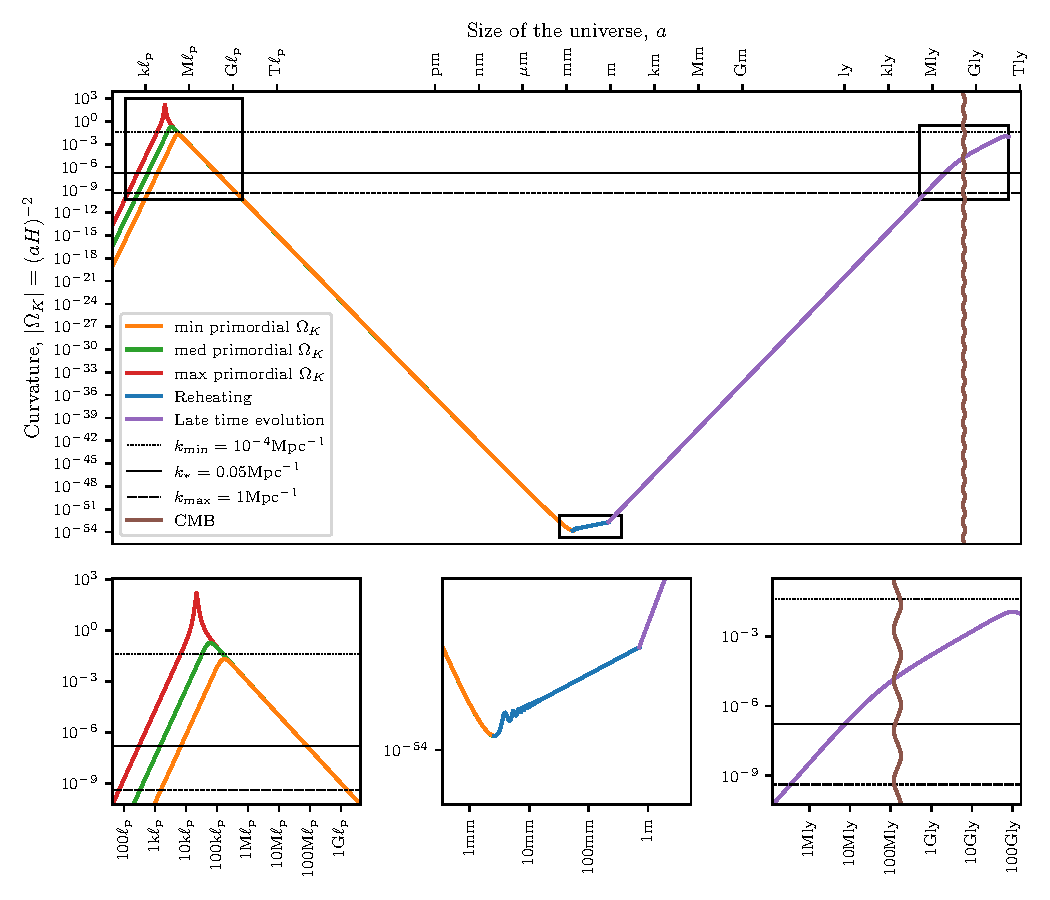
\includegraphics[width=0.49\textwidth]{figures/phi4o3}
        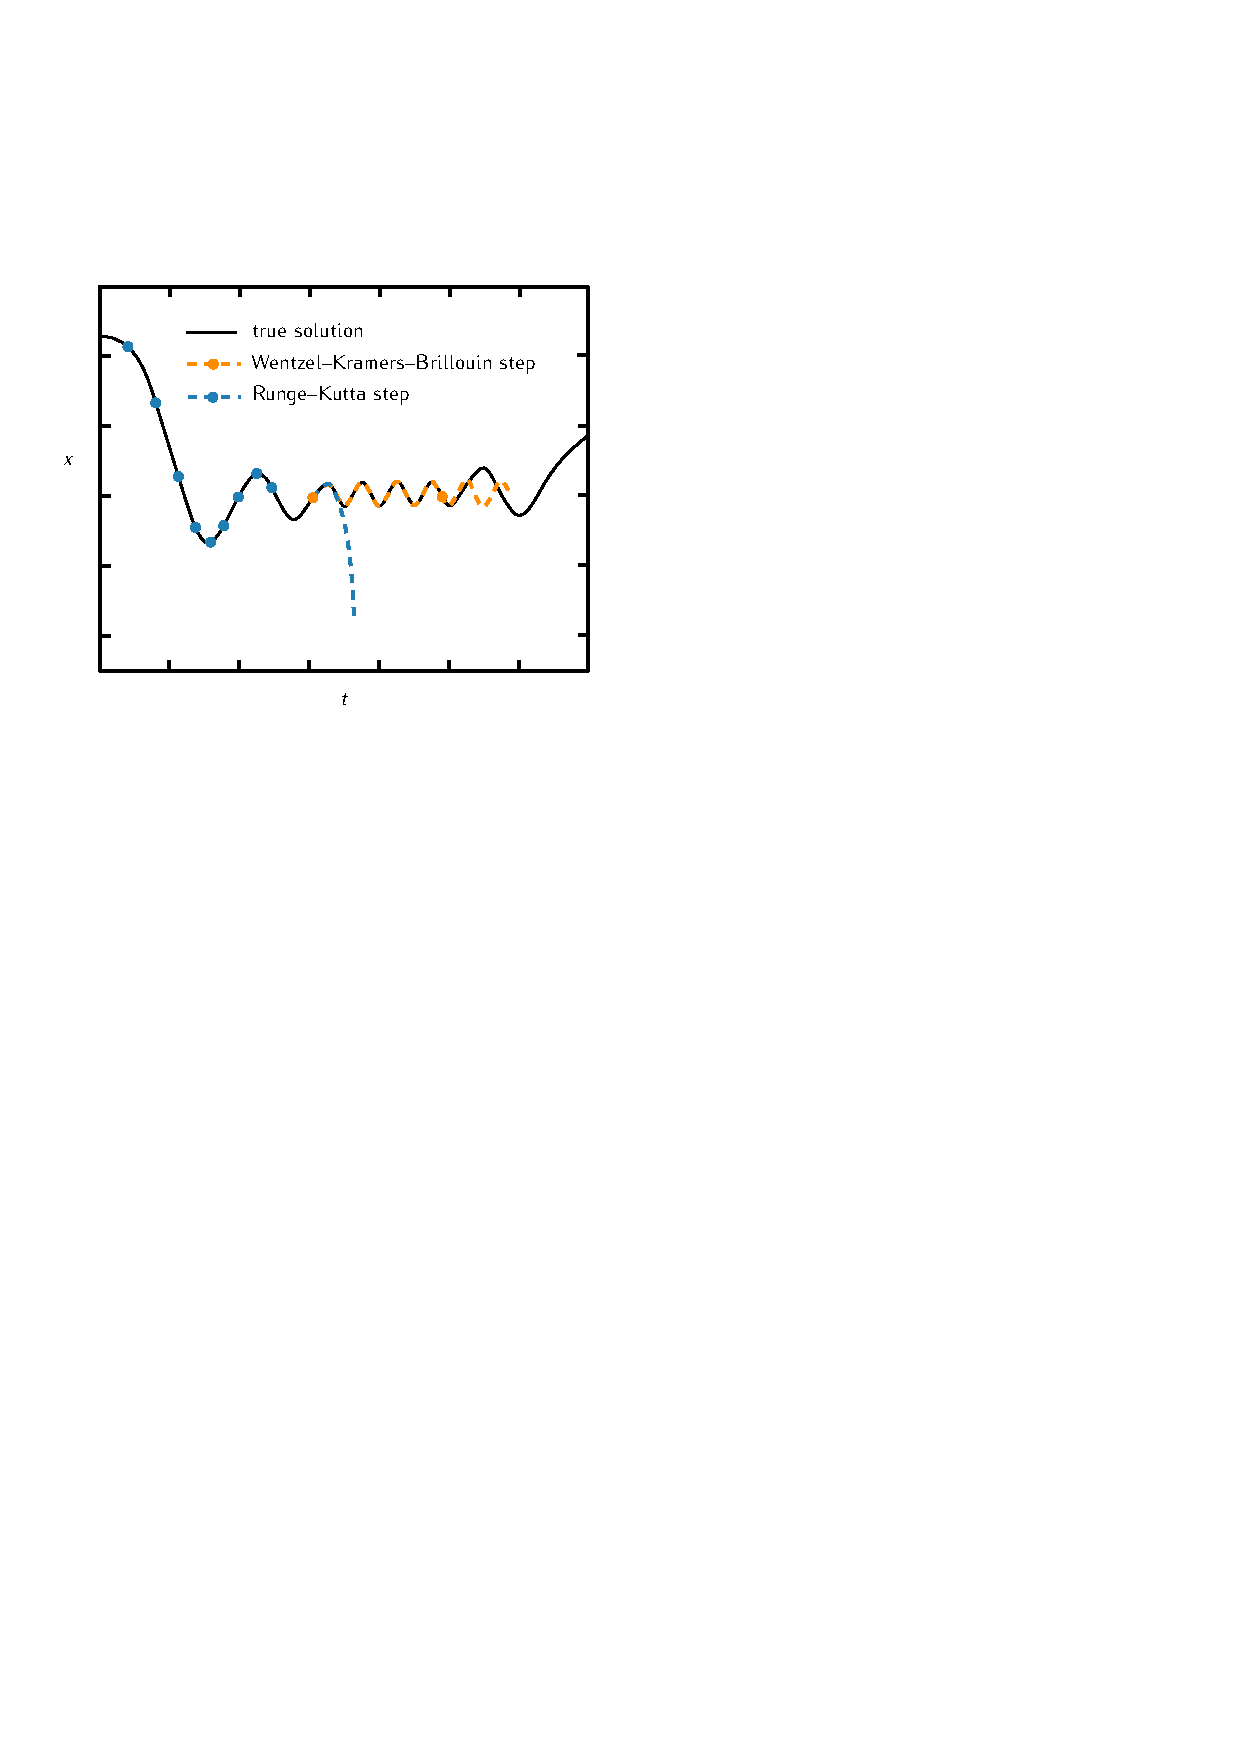
\includegraphics[width=0.49\textwidth]{figures/oscode}
        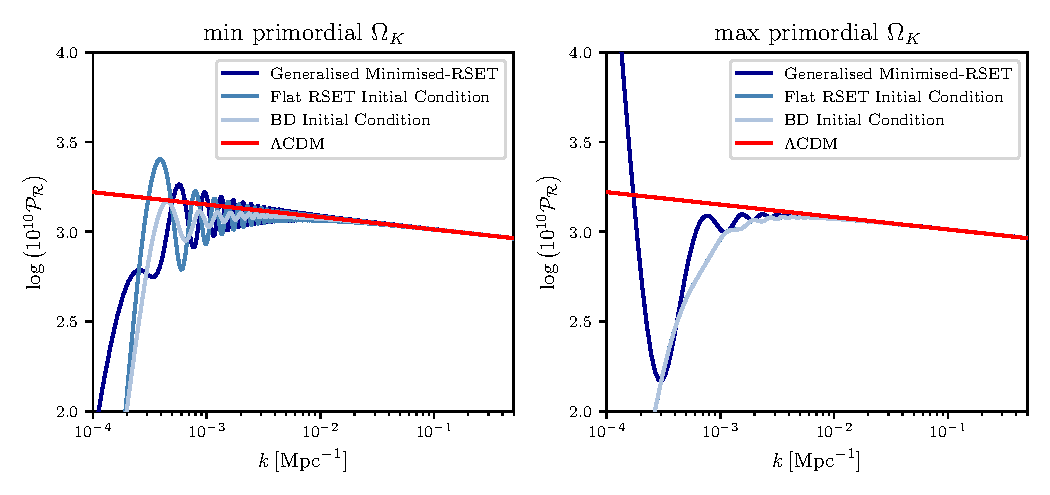
\includegraphics[width=0.49\textwidth]{figures/R-RST-flat-BD.pdf}
        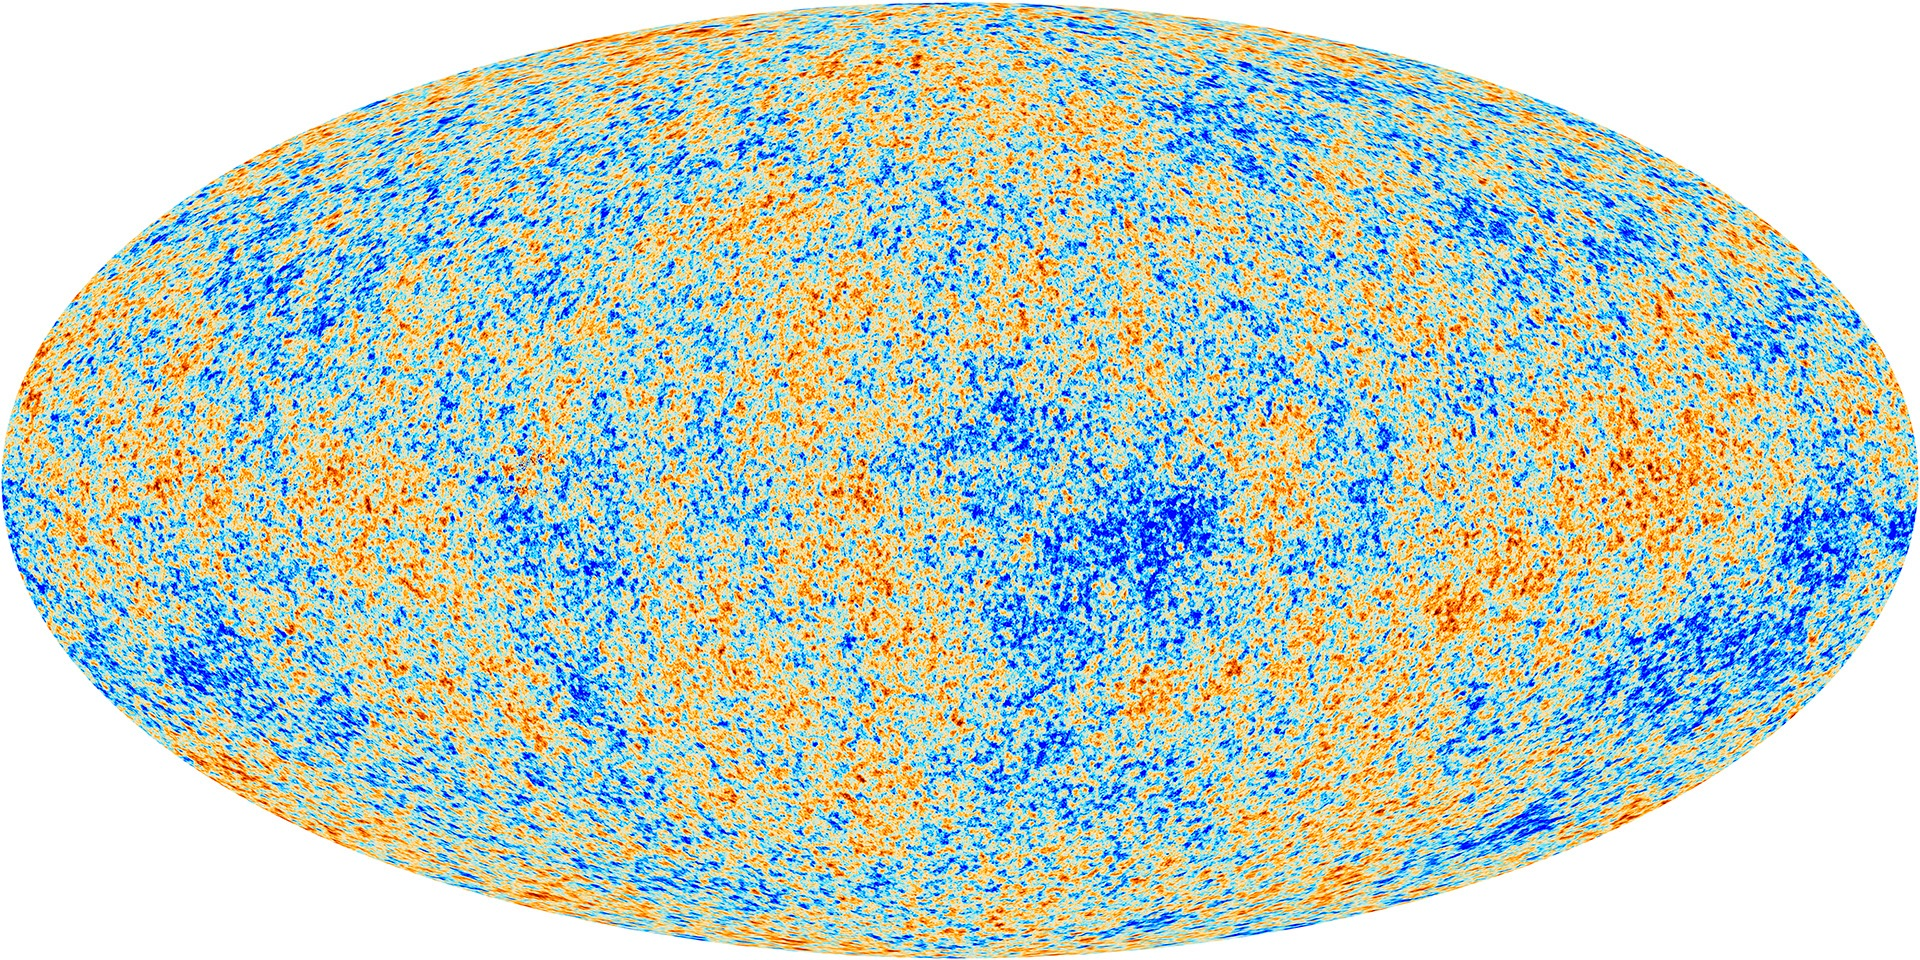
\includegraphics[width=0.49\textwidth]{figures/CMB.png}
    \end{columns}


\end{frame}

\begin{frame}
    \frametitle{Observation: REACH \& GAMBIT}
    \begin{columns}
        \column{0.6\textwidth}
        \begin{tabular}{lp{5cm}}
            \raisebox{-.7\totalheight}{
                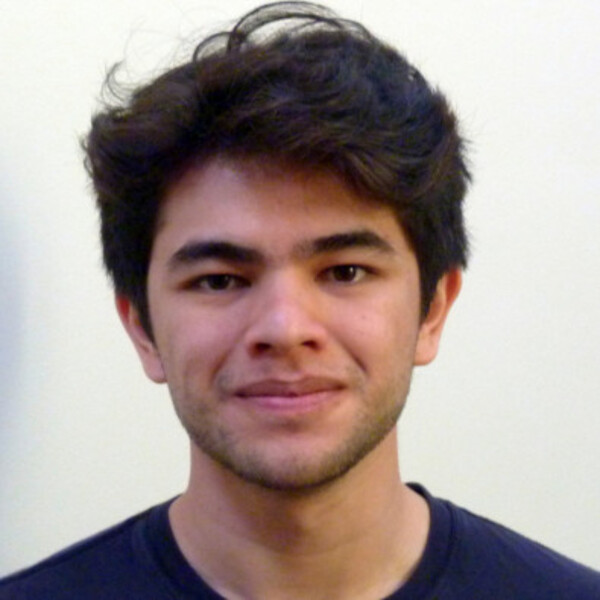
\includegraphics[width=50px]{images/ian_roque.jpg}%
                \begin{minipage}[b]{25px}
                    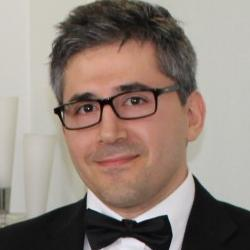
\includegraphics[width=25px]{images/nima_razavi_ghods.jpg} 
                \end{minipage}
            }&
            \textbf{Ian Roque} (PhD4) \newline
            Bayesian radiometer calibration for the REACH radio telescope.
            \\

            \raisebox{-.7\totalheight}{
                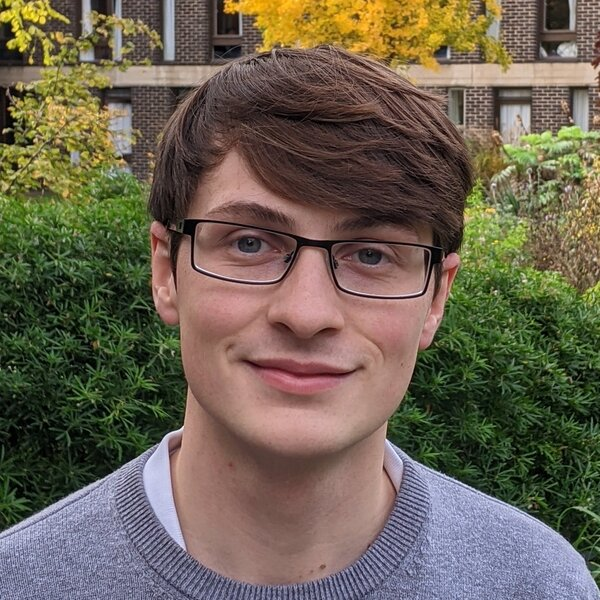
\includegraphics[width=50px]{images/thomas_gessey-jones.jpg}%
                \begin{minipage}[b]{25px}
                    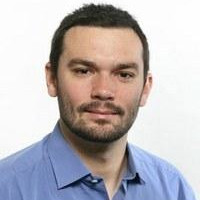
\includegraphics[width=25px]{images/eloy_de_lera_acedo.jpg}\vspace{-1px} 
                    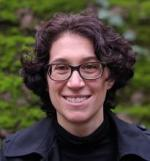
\includegraphics[width=25px]{images/anastasia_fialkov.jpg}%
                \end{minipage}
            }&
            \hspace{-4pt}\textbf{Thomas~Gessey-Jones}~(PhD3) \newline
            REACH 21cm universe theory: Pop III stars \& cosmic rays.
            \\

            \raisebox{-.7\totalheight}{
                
\includegraphics[width=50px]{images/harry_bevins.jpg}%
                \begin{minipage}[b]{25px}
                    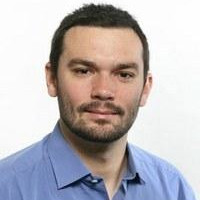
\includegraphics[width=25px]{images/eloy_de_lera_acedo.jpg}\vspace{-1px} 
                    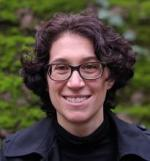
\includegraphics[width=25px]{images/anastasia_fialkov.jpg}%
                \end{minipage}
            }&
            \textbf{Harry Bevins} (PhD4) \newline
            21cm data analysis and machine learning:
            \texttt{margarine}, \texttt{maxsmooth} \& \texttt{globalemu}.
            \\


            \raisebox{-.7\totalheight}{
                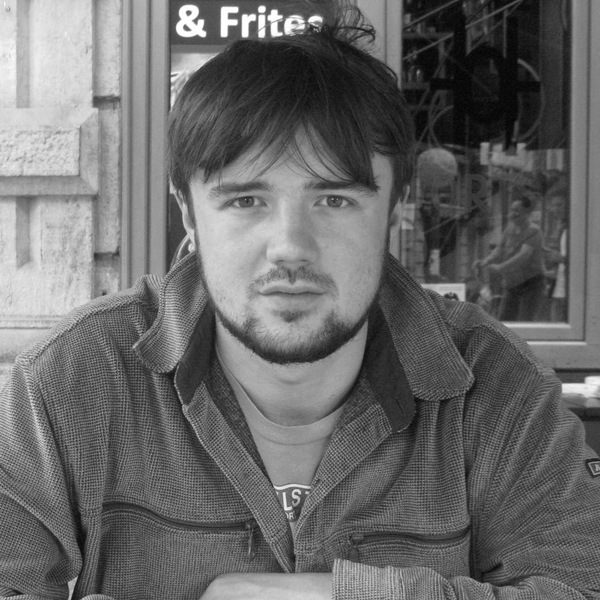
\includegraphics[width=50px]{images/sam_leeney.jpg}%
                \begin{minipage}[b]{25px}
                    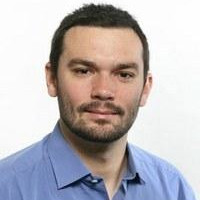
\includegraphics[width=25px]{images/eloy_de_lera_acedo.jpg}%
                \end{minipage}
            }&
            \textbf{Sam Leeney} (MPhil) \newline
            Bayesian RFI excision for REACH and pulsars.
            \\
        \end{tabular}

        \column{0.4\textwidth}
        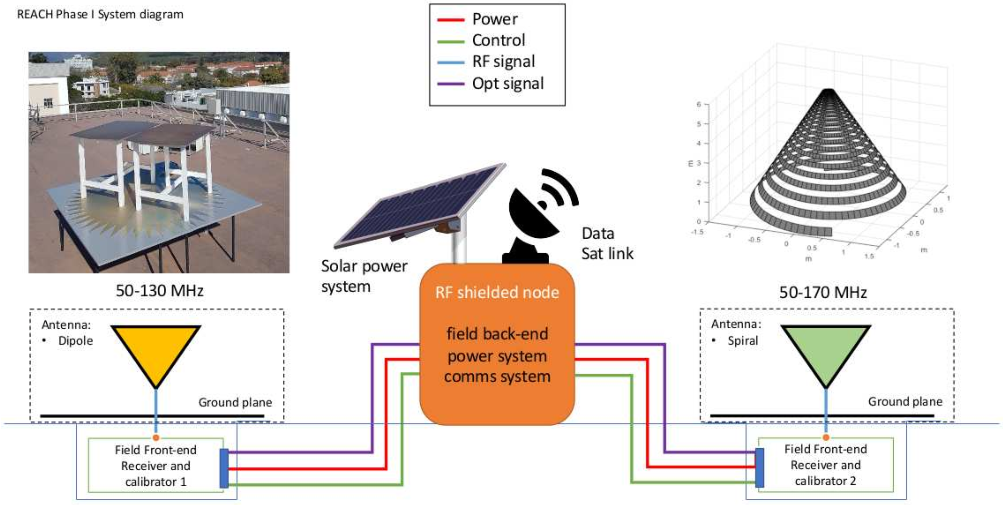
\includegraphics[width=\textwidth]{figures/reach_system.pdf}
        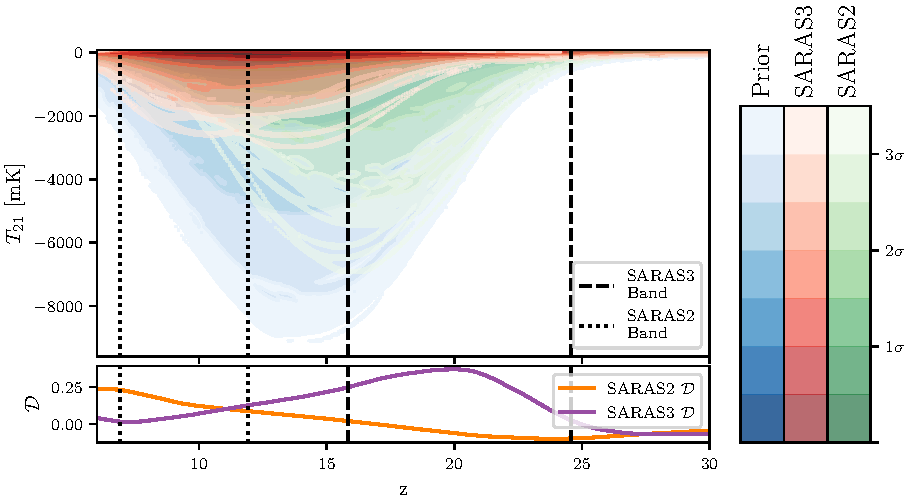
\includegraphics[height=0.31\textwidth]{figures/saras.pdf}
        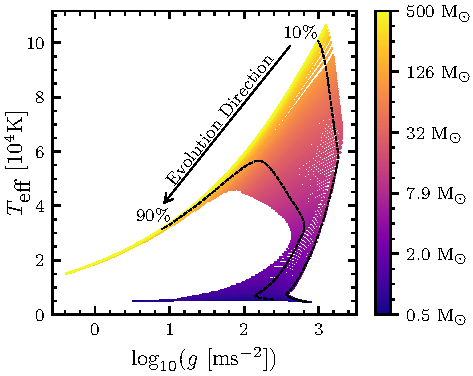
\includegraphics[height=0.31\textwidth]{figures/popIII.pdf}
        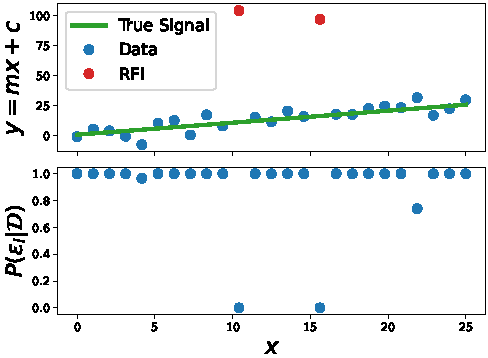
\includegraphics[height=0.22\textwidth]{figures/rfi3.pdf}
        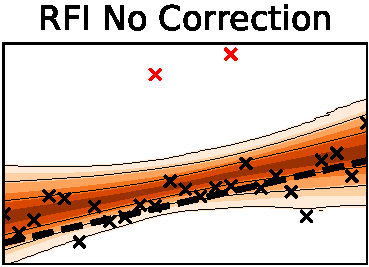
\includegraphics[height=0.22\textwidth]{figures/rfi1.pdf}
        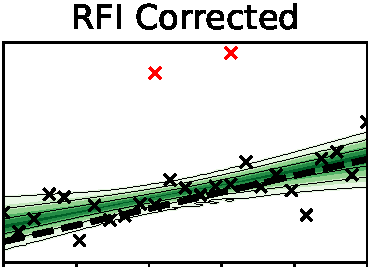
\includegraphics[height=0.22\textwidth]{figures/rfi2.pdf}
    \end{columns}
\end{frame}

\begin{frame}
    \frametitle{Inference: Nested sampling and Bayesian machine learning}
    \begin{columns}
        \column{0.6\textwidth}
        \begin{tabular}{lp{5cm}}
            \raisebox{-.7\totalheight}{
                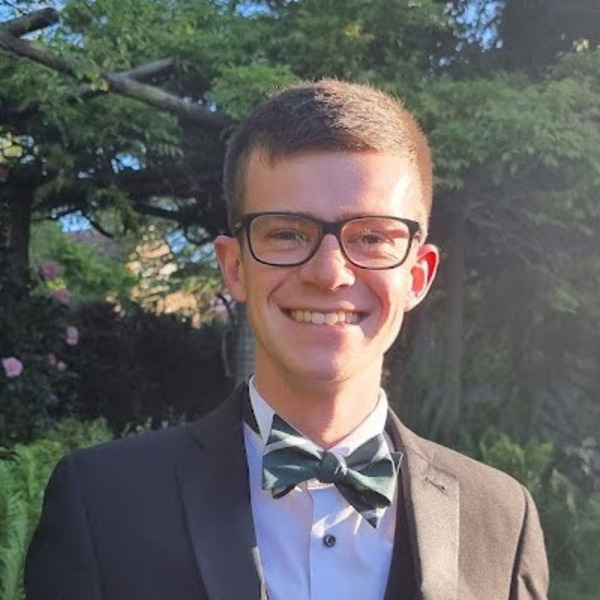
\includegraphics[width=50px]{images/adam_ormondroyd.jpg}%
                \begin{minipage}[b]{25px}
                    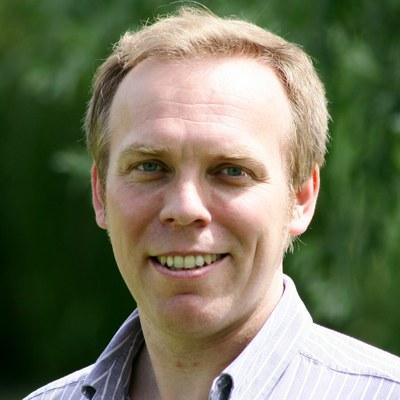
\includegraphics[width=25px]{images/mike_hobson.jpg}\vspace{-1px} 
                    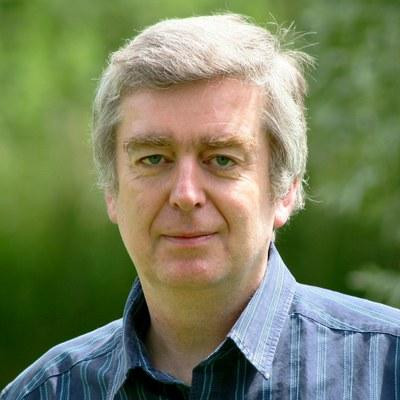
\includegraphics[width=25px]{images/anthony_lasenby.jpg}
                \end{minipage}
            }&
            \textbf{Adam Ormondroyd} (PhD2) \newline
            Cosmic history reconstructions, clustering in nested sampling.
            \\

            \raisebox{-.7\totalheight}{
                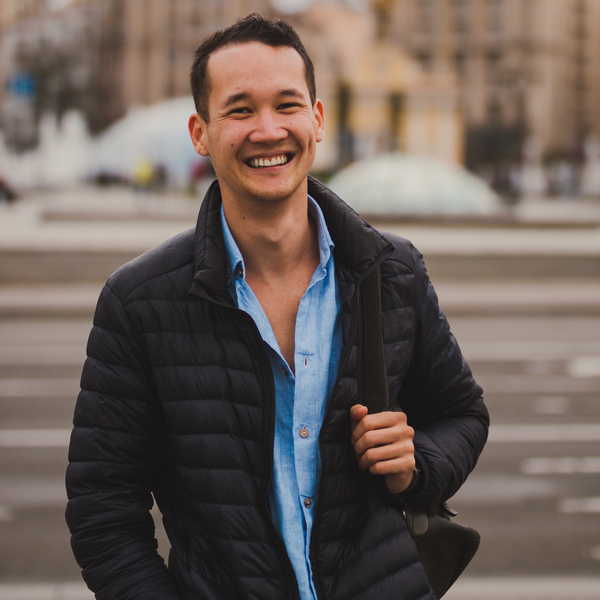
\includegraphics[width=50px]{images/kilian_scheutwinkel.jpg}%
                \begin{minipage}[b]{25px}
                    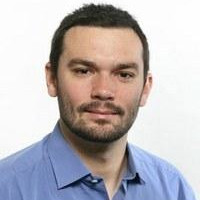
\includegraphics[width=25px]{images/eloy_de_lera_acedo.jpg}%
                \end{minipage}
            }&
            \textbf{Kilian Scheutwinkel} (PhD2) \newline
            Likelihood-free inference and nested sampling
            \\

            \raisebox{-.5\totalheight}{
                
\includegraphics[width=50px]{images/george_carter.jpg}%
                \begin{minipage}[b]{25px}
                    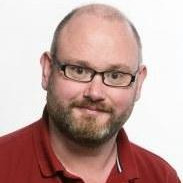
\includegraphics[width=25px]{images/mark_ashdown.jpg}\vspace{-1px}
                    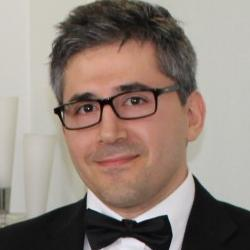
\includegraphics[width=25px]{images/nima_razavi_ghods.jpg}%
                \end{minipage}
            }&
            \textbf{George Carter} (PhD3) \newline 
            Bayesian global sky modelling
            \\

            \raisebox{-.7\totalheight}{
                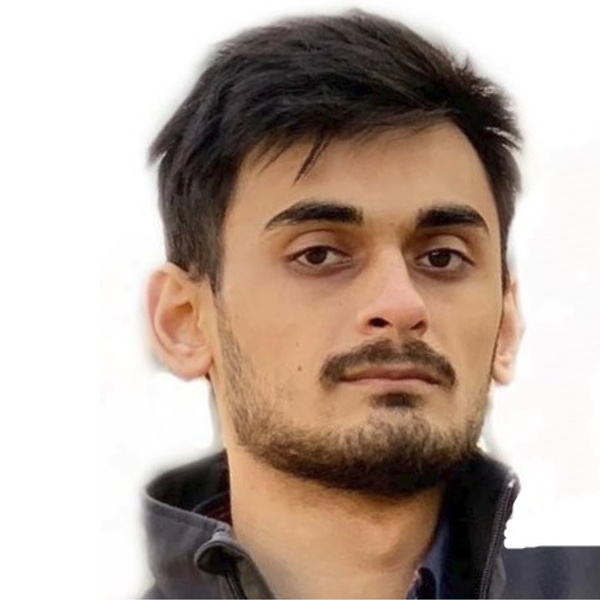
\includegraphics[width=50px]{images/allahyar_sahibzada.jpg}
            }&
            \textbf{Sahibzada Allahyar} (MPhil) \newline
            High-precision nested sampling, gravitational wave astrometry.
            \\
        \end{tabular}

        \column{0.4\textwidth}
        \includegraphics[height=0.9\textwidth]{figures/tmnre0.pdf}
        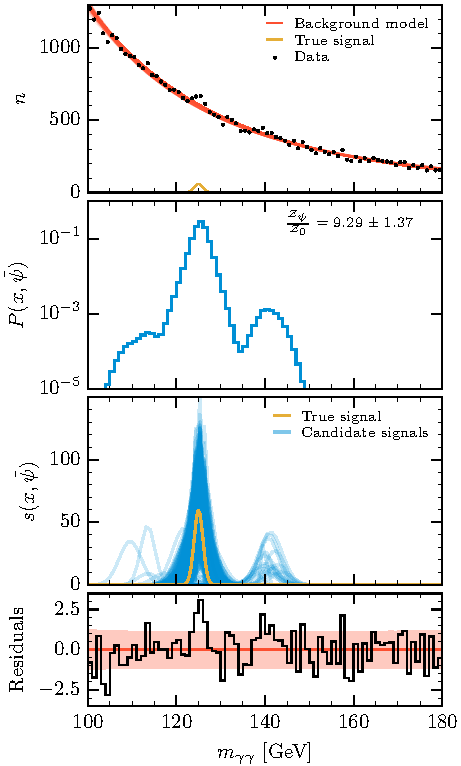
\includegraphics[height=0.9\textwidth]{figures/bumphunt.pdf}
        \begin{tabular}{lp{3.7cm}}
            \raisebox{-.8\totalheight}{
                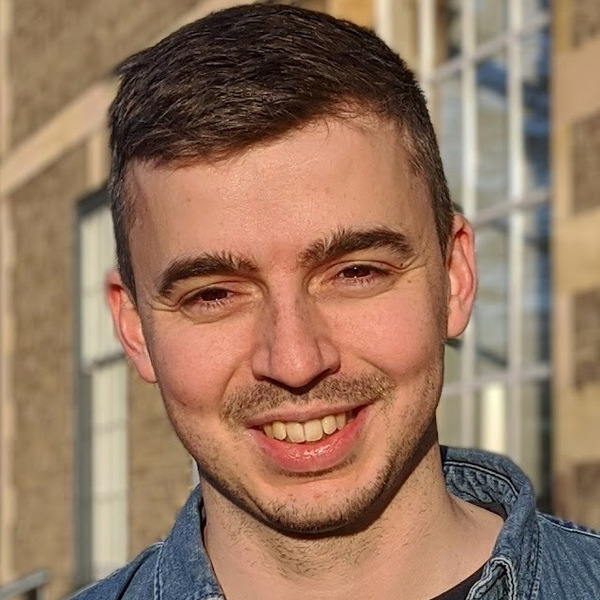
\includegraphics[width=50px]{images/david_yallup.jpg}%
            }&
            \hspace{-10pt}\textbf{David Yallup} (PostDoc) \newline
            Bayesian Neural Nets, sparse reconstruction, \& Gaussian Processes\\
        \end{tabular}
    \end{columns}

\end{frame}

\end{document}
